\documentclass[conference]{IEEEtran}
\usepackage{amsmath}
\usepackage{amsthm}
\usepackage{cite}
\usepackage{graphicx}
\usepackage[colorlinks=True, allcolors=blue]
{hyperref}
\usepackage{booktabs}
\usepackage{caption}



\begin{document}

\title{Analysis and Time Series Forecasting of Sales for ``NOR TUN'' Chain Stores}

\author{
    \IEEEauthorblockN{Naira Maria Barseghyan}
    \IEEEauthorblockA{BS in Data Science\\
    American University of Armenia\\
    Email: naira\_barseghyan@edu.aua.am}
    \and
    \IEEEauthorblockN{Supervisor: Natali Gzraryan}
    \IEEEauthorblockA{American University of Armenia\\
    Email: gzraryannatali@gmail.com}
}

\maketitle


%  =====================================================================================================================================
%                                                        Abstract
%  =====================================================================================================================================
\begin{abstract}
This paper leverages sales data of ``NOR TUN'' chain stores provided by BARSIS LLC to conduct wide research, perform detailed sales analysis, and implement forecasting methods to predict future sales of the company. Analysis of sales data is widely used in business. It can provide valuable information about the performance of the business and can be used to identify strengths and weaknesses of the business. Visualization tools were used for the business analysis. The analysis found the best-performing products and brands of the stores. A comparison of stores was done based on their geographical location. In the scope of this research, various classical and modern Time Series Forecasting techniques were used to construct accurate forecasting models that can potentially benefit the business. Univariate and multivariate forecasting methods were used to make predictions for both the company’s overall sales and for specific shops in the chain stores. Before processing to forecasting, feature engineering steps were conducted to improve the forecasting result. For univariate forecasting, custom LSTM models were implemented and evaluated, but they did not show desirable results. The best model for univariate forecasting was the transformer-based Lag-Llama pre-trained model. This model was fine-tuned on the training part of data and later was evaluated on unseen data. The zero-shot capabilities of this model were tested and used as a benchmark for the evaluation of the fine-tuned model. Finally, machine learning models were implemented for multivariate forecasting. Five models, including regression and ensemble models, were evaluated. Based on the evaluation, two best-performing models were used with the ensemble technique and combined in the Stacking Regressor model. Stacked models were expected to perform better than base models; however, after evaluation, it was found that the best model for multivariate analysis is the Random Forest Regressor, which shows again that the often simplest solution is the best solution. The evaluation for models was done using Mean Absolute Error (MAE), Mean Absolute Percentage Error (MAPE), Root Mean Squared Error (RMSE), and R-squared metrics. The findings of the project aim to contribute to strategic planning of the business, investment decisions, and inventory management.
\end{abstract}
\begin{IEEEkeywords}
Sales Analysis, Time Series Forecasting, LSTM, Transformer model, Lag-Llama, Fine-Tuning, Stacking Regressor, Random Forest Regressor, XGBoost Regressor
\end{IEEEkeywords}


%  =====================================================================================================================================
%                                                        Introduction
%  =====================================================================================================================================

\section{Introduction}
Sales analysis is an important tool for business development, providing insights into the performance of the business. By examining sales data, stakeholders can identify the businesses strengths and weaknesses, which guides decision-making process and future investment strategies. Another method of enhancing business performance is using modern technologies to predict future sales. For that reason, time series forecasting is used. In retail, time series sales forecasting (TSSF) helps the merchants to manage their inventory scientifically.\cite{alibaba_arxiv} In the TSF field, various methods are used to generate accurate results. Businesses that can find the best methods to use the accumulated historical data are gaining a competitive advantage in the field. Various techniques are used for forecasting, such as deep neural networks, Machine Learning algorithms, and transformer-based models. In recent years, the growing attention to the transformer models has encouraged researchers to adapt the transformer models for forecasting. This research aims to:
\begin{enumerate}
    \item Analyze the existing historical data of the business in order to find interesting patterns and provide a deep understanding of the performance of various aspects related to sales.
    \item Build and analyze various TSF methods and identify the best technique to forecast sales of the ``Nor Tun'' chain store.
\end{enumerate}
For the first part of the research, visualization tools were used, more specifically, R programming language along with the ggplot library. The models used include a Long Short-Term Memory (LSTM) neural network, which is known to perform well on sequential data. Originally, LSTMs were used to model textual data; however, after discovering their ability to perform well on all types of sequential data, they were leveraged in the TSF field and outperformed classical ARIMA models. Next, ML regression algorithms were tested to find the best-performing regression models, which were later used together using the Stacking Regressor. Finally, the newest pre-trained transformer model called Lag-Llama was fine-tuned on ``Nor Tun'' data and used for forecasting. Each model was evaluated to determine its efficacy in a real-world business context. The following sections will dive deeper into data preparation, business analysis, and the mentioned algorithms.

%  =====================================================================================================================================
%                                                        Related Work
%  =====================================================================================================================================
\section{Related Work}
Time series forecasting is an important topic for researchers. New methods for forecasting are being produced every year. TSF is also a very useful tool for real-life businesses. Given these facts, there are various papers that discuss TSF specifically for sales prediction. The paper that encouraged this project is ``From Known to Unknown: Knowledge-guided Transformer for Time-Series Sales Forecasting in Alibaba,'' written by scientists at Alibaba.\cite{alibaba_arxiv} Scientists working for Alibaba have implemented the TSF transformer model that is being used in the business. This paper was the motivation for exploring the transformer-based models for TSF on real-world sales data. As a result, the Lag-Llama transformer-based model was fine-tuned and used in this research.\cite{lag_llama_arxiv}

The next notable paper is ``Lag-Llama: Towards Foundation Models for Probabilistic Time Series Forecasting''. This paper describes the architecture of the Lag-Llama model designed for univariate forecasting, which is used in this research.\cite{lag_llama_arxiv}

The paper ``Predicting Future Sales of Retail Products using Machine Learning'' explores XGBoost and LSTM algorithms for TSF.\cite{sales_prediction} This paper was useful since the field of study was very similar to the field of study of my research. From this paper, I have gained understanding about models that can be useful for my study, and later leveraged them.

%  =====================================================================================================================================
%                                                       Data
%  =====================================================================================================================================

\section{Data}
% Please add the following required packages to your document preamble:

\begin{table}[]
\centering
\resizebox{\columnwidth}{!}{%
\begin{tabular}{|l|l|l|}
\hline
\textbf{Attribute}            & \textbf{Description}                                                                                  & \textbf{DataType} \\ \hline
\textbf{sale\_date}           & \begin{tabular}[c]{@{}l@{}}The date on which \\ the sale occurred.\end{tabular}                       & Date              \\ \hline
\textbf{Revenue\_VAT}         & \begin{tabular}[c]{@{}l@{}}The revenue from the sale \\ including value-added tax.\end{tabular}       & numeric           \\ \hline
\textbf{Quantity}             & \begin{tabular}[c]{@{}l@{}}The number of units sold \\ in each transaction.\end{tabular}              & numeric           \\ \hline
\textbf{product\_type}        & \begin{tabular}[c]{@{}l@{}}The type or category of the \\ product sold.\end{tabular}                  & character         \\ \hline
\textbf{Brand}                & The brand of the product.                                                                             & character         \\ \hline
\textbf{manufacture\_country} & \begin{tabular}[c]{@{}l@{}}The country where the \\ product was manufactured.\end{tabular}            & character         \\ \hline
\textbf{Branch}               & \begin{tabular}[c]{@{}l@{}}The store where the sale \\ took place.\end{tabular}                       & character         \\ \hline
\textbf{City}                 & \begin{tabular}[c]{@{}l@{}}The city in which the \\ branch is located.\end{tabular}                   & character         \\ \hline
\textbf{Districts}            & \begin{tabular}[c]{@{}l@{}}The district of Yerevan \\ where the branch is located.\end{tabular}       & character         \\ \hline
\textbf{Regions}              & \begin{tabular}[c]{@{}l@{}}The region of Armenia \\ where the branch location.\end{tabular}           & character         \\ \hline
\textbf{Product\_category}    & \begin{tabular}[c]{@{}l@{}}The broader category to \\ which the product belongs.\end{tabular}         & character         \\ \hline
\textbf{IsHoliday} &
  \begin{tabular}[c]{@{}l@{}}A binary indicator (0 or 1) \\ denoting whether the sale \\ occurred on a holiday.\end{tabular} &
  integer \\ \hline
\textbf{month}                & \begin{tabular}[c]{@{}l@{}}The month when the \\ sale occurred.\end{tabular}                          & numeric           \\ \hline
\textbf{year}                 & \begin{tabular}[c]{@{}l@{}}The year when the \\ sale occurred.\end{tabular}                           & numeric           \\ \hline
\textbf{day}                  & \begin{tabular}[c]{@{}l@{}}The day of the month on \\ which the sale took place.\end{tabular}         & integer           \\ \hline
\textbf{day\_of\_week} &
  \begin{tabular}[c]{@{}l@{}}The day of the week \\ represented numerically \\ (e.g.,1 for Monday, \\ 2 for Tuesday, etc.).\end{tabular} &
  numeric \\ \hline
\textbf{day\_name} &
  \begin{tabular}[c]{@{}l@{}}The name of the day on \\ which the sale took place \\ (e.g., Monday, Tuesday).\end{tabular} &
  character \\ \hline
\textbf{quarter}              & \begin{tabular}[c]{@{}l@{}}The quarter of the year\\  during which the sale \\ occurred.\end{tabular} & integer           \\ \hline
\textbf{is\_weekend} &
  \begin{tabular}[c]{@{}l@{}}A numeric indicator (0 or 1) \\ denoting whether the sale \\ occurred on a weekend.\end{tabular} &
  numeric \\ \hline
\textbf{week\_of\_year} &
  \begin{tabular}[c]{@{}l@{}}The specific week of \\ the year during which \\ the sale took place.\end{tabular} &
  numeric \\ \hline
\textbf{sales\_proxy\_week} &
  \begin{tabular}[c]{@{}l@{}}The average weekly sales \\ revenue, adjusted for each \\ branch and week.\end{tabular} &
  numeric \\ \hline
\textbf{sales\_proxy\_month} &
  \begin{tabular}[c]{@{}l@{}}The average monthly sales \\ revenue, adjusted for each \\ branch and month.\end{tabular} &
  numeric \\ \hline
\end{tabular}%
}
%\captionsetup[table]{skip=100pt}
\caption{ Attributes and Descriptions of Sales Data for 'NOR TUN' Chain Stores}
\label{tab:attribute_table}
\end{table}
I would like to acknowledge the company BARSIS LLC,  which provided the sales data for the “Nor Tun” chain stores. To further enhance the research, other information was added to the original data. This added information includes the cities of Armenia and the Districts of Yerevan where the stores operate. The purpose of adding this information was to find out the performance of the shops depending on the geographical area. 

%  =====================================================================================================================================
%                                                       Data Exploration
%  =====================================================================================================================================

\subsection{Data Exploration}
The following figures will help to understand the data, and the relationship between attributes better. In~\autoref{tab:attribute_table}  description of data can be found.

There are 15 product categories and 285 Brands, 24 manufacturer countries. The regional columns, city, districts and regions are identifying the geographical location of stores. These attributes are explored in the Business analysis section.

%  =====================================================================================================================================
%                                                       Data Cleaning and Translation
%  =====================================================================================================================================

\subsection{Data Cleaning and Translation}
The provided data needed to pass multiple preprocessing steps before it could be used for visualizations and modeling. The provided data was in the Excel format (.xlsx), and because of the specific way that the data is rendered from the “1C” accounting program, files were not accessible for any other program except Excel.
It was not possible to convert the files into csv format or read the files using R or Python programming languages. Issue was resolved by finding, the rendering issue was found and corrected using Python. 
The next step was the translation of the data from Armenian to English. This was an important aspect since the research and analysis were done in English, and data needed to be interpretable for English readers. Google Translate API was used for the translation. After acquiring translations of all unique textual information, the translations were stored in a Python dictionary and later used to translate the whole dataset. The translated columns were manufacturer country, shop, brand, and product names. During this step, the shop addresses were mapped with their geographic location, where the city and district of the shops were specified. 
The general approach for handling missing values is to replace them with other meaningful values, such as the average of existing values. However, this was not an appropriate approach for this specific case since the sales vary based on the product type, brand, and the shop in which the sale happened. The most sensible approach was to find the average of the specific product sold in the specific shops; however, after deeper inspections, it was found that for the missing values in the revenue, other specifications of the sale were missing as well, which made the replacement of the missing values with meaningful values impossible. Therefore, the full removal of the missing values was chosen. This did not affect the quality of the analysis since the amount of missing values was not significant. The original data had around 1.5 million entries, out of which 709 were missing values. Since the missing values were less than half a percent of the data, the elimination of missing values is not a significant loss.

%  =====================================================================================================================================
%                                                      Feature Engineering
%  =====================================================================================================================================

\subsection{Feature Engineering}
The original data did not contain the following attributes. The attributes IsHoliday, month, year, day, day\_of\_week, day\_name, quarter, is\_weekend, week\_of\_year, sales\_proxy\_week, and sales\_proxy\_month were added to the data in order to get additional variables that can potentially affect the quality of the prediction. This process is known as feature engineering, which is when features are added and transformed, which leads the model to capture interesting patterns in data. The IsHoliday column is added to show the official non-working holiday days in Armenia. Other time-dependent variables (day, year, quarter, is\_weekend, week\_of\_year) were added to capture the effect of specific time frames on the sales. The sales\_proxy\_week and sales\_proxy\_month columns are added to catch temporal trends and seasonal patterns more effectively while doing multivariate analysis. Proxy columns are the average sales revenue of the specific month or week across all years, adjusted for each branch.


\begin{figure}[htbp]
\centering
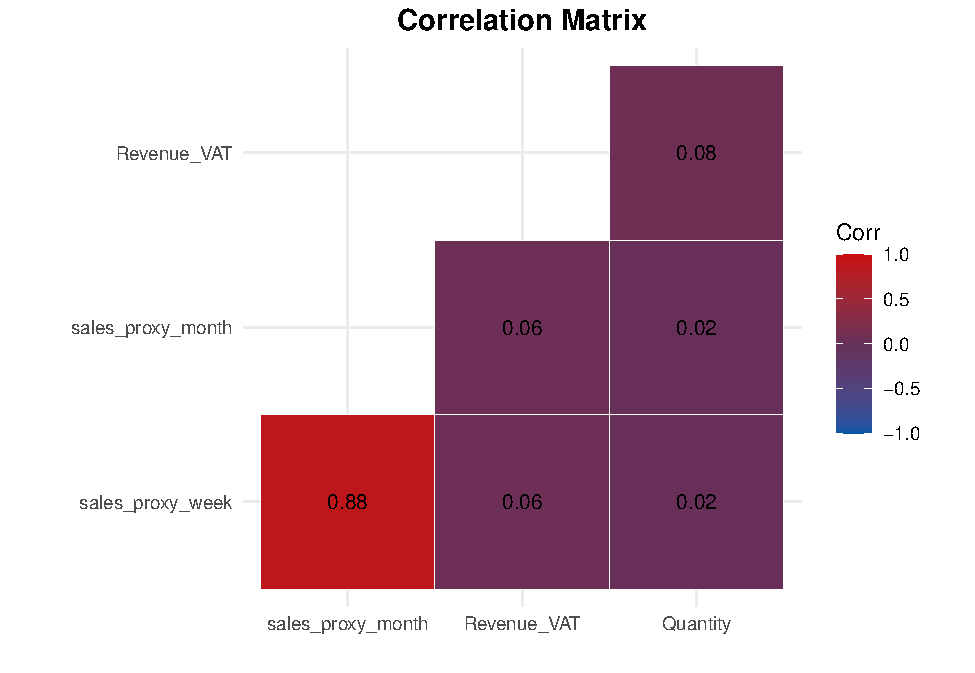
\includegraphics[width=\columnwidth,keepaspectratio]{./figures/correlation_matrix_with_style.pdf}
\caption{ Correlation Matrix for Sales Continuous Variables \cite{correlation}}
\label{fig:correlationMatrix}
\end{figure}
The relationship between continuous variables was examined by computing the correlation matrix. Figure~\ref{fig:correlationMatrix} suggests that there is no significant relationship between revenue and added proxy features. Despite the low correlation score, proxy features increased the accuracy of the model, and the final decision was to keep the proxy features. 

% Please add the following required packages to your document preamble:
% \usepackage{booktabs}
% \usepackage{graphicx}
\begin{table}[]
\centering
\resizebox{\columnwidth}{!}{%
\begin{tabular}{@{}lllllll@{}}
\toprule
\textbf{Factor}               & \textbf{Df} & \textbf{SumSq} & \textbf{MeanSq} & \textbf{Fvalue} & \textbf{Pr} & \textbf{Significance} \\ \midrule
\textbf{product\_type}  & 199 & 3.7e+15 & 1.8e+13 & 4.1e+03 & 0.0e+00  & *** \\
\textbf{Brand}          & 284 & 2.0e+15 & 7.0e+12 & 1.2e+03 & 0.0e+00  & *** \\
\textbf{manufacture\_country} & 23          & 8.5e+14        & 3.7e+13         & 5.8e+03         & 0.0e+00     & ***                   \\
\textbf{Branch}         & 24  & 3.2e+13 & 1.3e+12 & 1.9e+02 & 0.0e+00  & *** \\
\textbf{City}           & 11  & 7.7e+12 & 7.0e+11 & 1.0e+02 & 3.3e-232 & *** \\
\textbf{IsHoliday}      & 1   & 2.1e+11 & 2.1e+11 & 3.1e+01 & 2.5e-08  & *** \\
\textbf{day\_of\_week}  & 1   & 5.1e+11 & 5.1e+11 & 7.3e+01 & 1.0e-17  & *** \\
\textbf{week\_of\_year} & 1   & 4.7e+08 & 4.7e+08 & 6.9e-02 & 7.9e-01  &     \\
\textbf{is\_weekend}    & 1   & 1.2e+07 & 1.2e+07 & 1.8e-03 & 9.7e-01  &     \\
\textbf{quarter}        & 1   & 1.1e+10 & 1.1e+10 & 1.6e+00 & 2.0e-01  &     \\
\textbf{year}           & 1   & 1.4e+10 & 1.4e+10 & 2.0e+00 & 1.6e-01  &     \\
\textbf{month}          & 1   & 1.4e+10 & 1.4e+10 & 2.1e+00 & 1.5e-01  &     \\
\textbf{day}            & 1   & 4.2e+11 & 4.2e+11 & 6.1e+01 & 4.7e-15  & *** \\ \bottomrule
\end{tabular}%
}
%\captionsetup[table]{skip=100pt}
\caption{ANOVA Results for Sales Data by Different Factors}
\label{tab:anova-table}
\end{table}
In order to explore the relationship between attributes in the dataset,  a one-way ANOVA test was chosen. The dependent variable is the amount of revenue from each sale (Revenue\_VAT), while most of the independent variables are categorical. The one-way ANOVA test is the most reliable way to study the relationship between continuous and categorical variables. (Find details about Anova in Appendix~\autoref{app:anova}) In~\autoref{tab:anova-table}, detailed information about the ANOVA test between the dependent variable (Revenue\_VAT) and all categorical variables can be found. As we can see, the majority of attributes are highly correlated with dependent variables. Variables week\_of\_year, is\_weekend, quarter, year, and month are not affecting the dependent variable significantly.

%  =====================================================================================================================================
%                                                        Business Analysis
%  =====================================================================================================================================


\section{Business Analysis}
This section aims to explore the sales data, find patterns, and identify the best-performing aspects of stores.


%  =====================================================================================================================================
%                                                        Revenue Trends
%  =====================================================================================================================================

\subsection{Revenue Trends}
This section explores revenue trends of ``NOR TUN'' chain stores over the past three years, providing insights into the monthly and annual sales performance across different years. Revenue trends are essential for understanding the overall growth of the business and specific seasonal patterns of sales. The heatmap (Figure ~\ref{fig:heatmap}) shows a clear pattern of revenue changes across different months.
\begin{figure}[htbp]
\centering
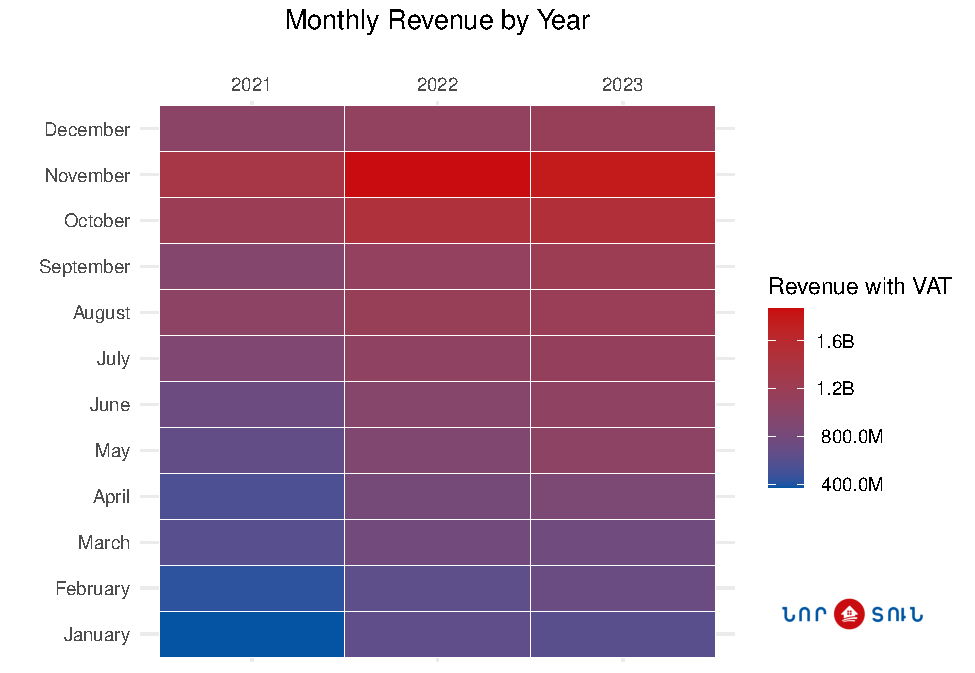
\includegraphics[width=\columnwidth,keepaspectratio]{./figures/heatmap_sales.pdf}
\caption{Heatmap of Monthly Revenue by Year\cite{heatmap}}
\label{fig:heatmap}
\end{figure}
There has been a noticeable increase in revenue in the last quarter of the year, particularly in November. This suggests that there is a strong seasonal impact on the revenue. The performance of November is connected to holiday shopping, more specifically to Black Friday. This pattern will be further examined in the Daily revenue trends section. The increase in revenue has also been noticeable across the years. This pattern can be seen more clearly on the Area graph (Figure~\ref{fig:area-graph}). Each consecutive year, revenue ranks higher compared to the previous year across almost all months. This suggests overall growth in revenue year-by-year.
\begin{figure}[htbp]
\centering
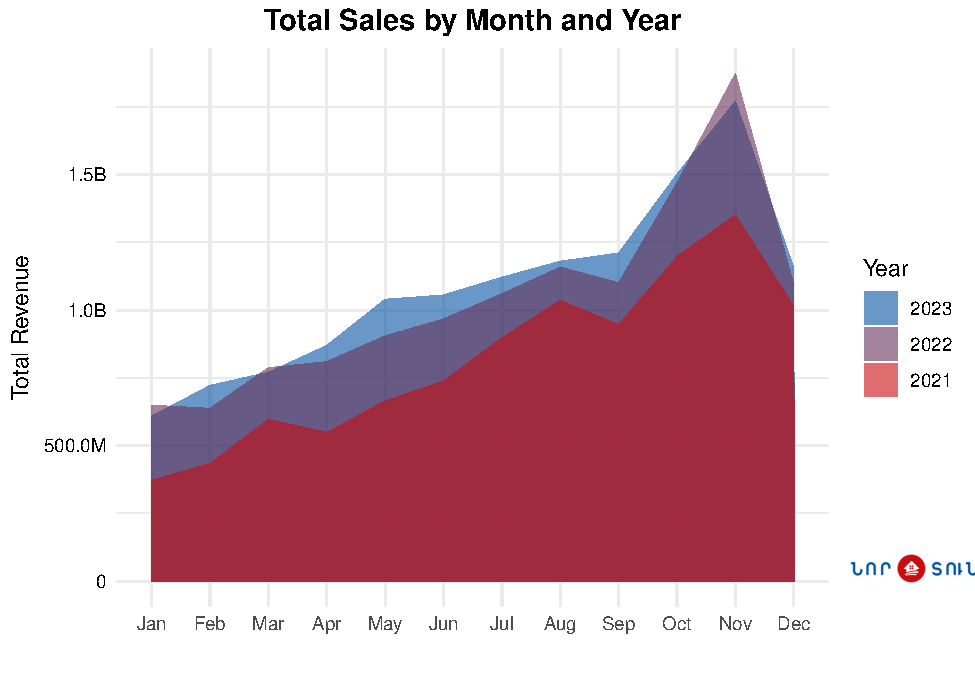
\includegraphics[width=\columnwidth,keepaspectratio]{./figures/area_graph_sales_by_year.pdf}
\caption{Area Graph of Total Sales by Month and Year \cite{area}}
\label{fig:area-graph}
\end{figure}

%  =====================================================================================================================================
%                                                       Daily Revenue Trends 
%  =====================================================================================================================================

\subsection{Daily Revenue Trends}
This section will explore revenue trends on a smaller scale to catch interesting patterns in day-to-day sales. Figure 4 shows the day-to-day revenue of stores in 2023. (The visualization of 2022 and 2021 can be found in Appendix~\autoref{app:time-series}). Across all three years, the spikes in sales are found near the end of the year. This is linked to the holiday promotions and specifically to Black Friday sales. Each year, stores announce big sales during the last week of November, which causes an increase in sales. 
\begin{figure}[htbp]
\centering
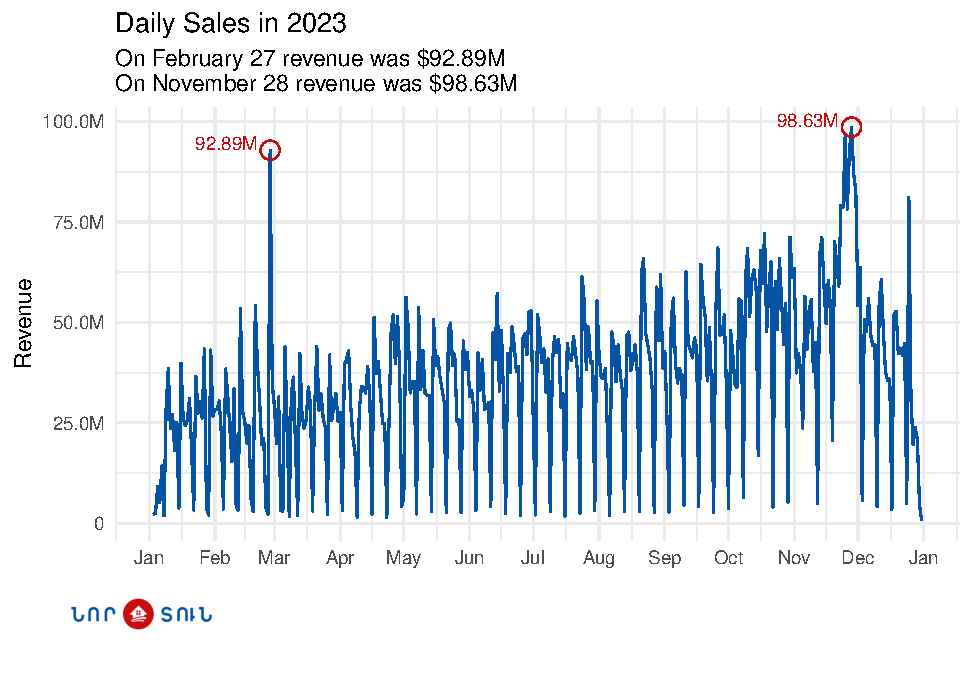
\includegraphics[width=\columnwidth,keepaspectratio]{./figures/time_series_2023_sales.pdf}
\caption{Daily Sales Trends for in 2023: Highlighting Sales Peaks \cite{TSF}}
\label{fig:time-series-2023}
\end{figure}
Interestingly, in 2023, there were two spikes in sales, and the first one did not occur at the expected time. This was an anomaly since there were no sales or specifically planned activities that could have caused this spike. It is noticeable from Figure~\ref{fig:time-series-2023} that sales have weekly seasonality. This pattern can be examined more clearly on Figure~\ref{fig:weekday}. The average sales by weekday show a clear pattern of weekly sales across all years. The sales are peaking on Monday, decreasing with every coming day, and are dropping on Sunday.

\begin{figure}[htbp]
\centering
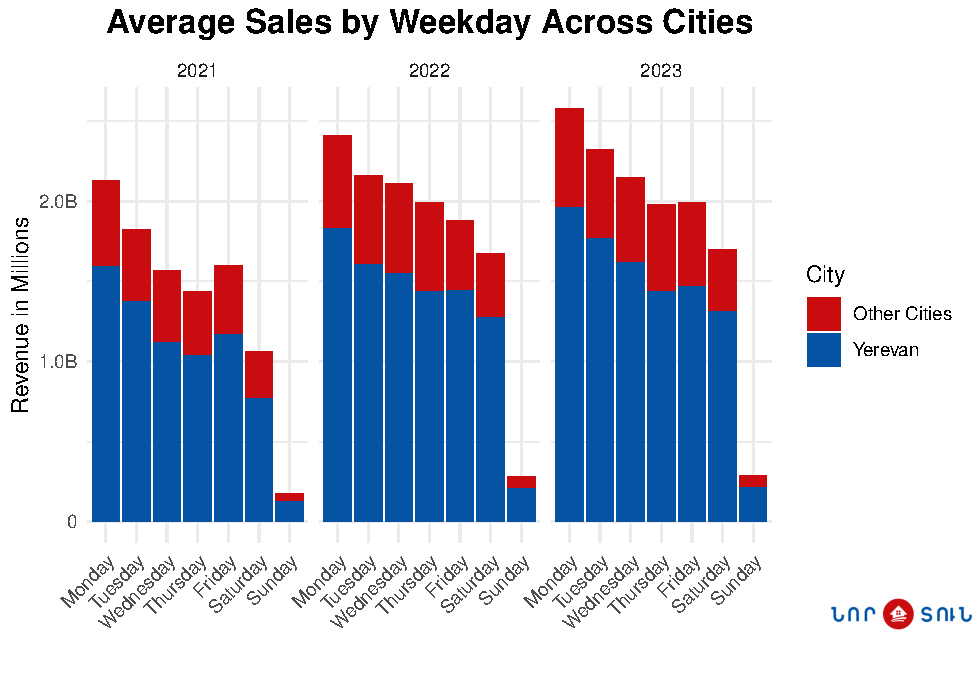
\includegraphics[width=\columnwidth,keepaspectratio]{./figures/sales_by_weekday.pdf}
\caption{Source \cite{weekly}}
\label{fig:weekday}
\end{figure}

%  =====================================================================================================================================
%                                                       Comparative Analysis Among Shops
%  =====================================================================================================================================

\subsection{Comparative Analysis Among Shops}
Revenue distribution across different shops is not symmetrical. Moreover, there is a significant divergence between shops in Yerevan and other cities. This can be clearly observed from Figure~\ref{fig:treemap_whole}. 

\begin{figure}[htbp]
\centering
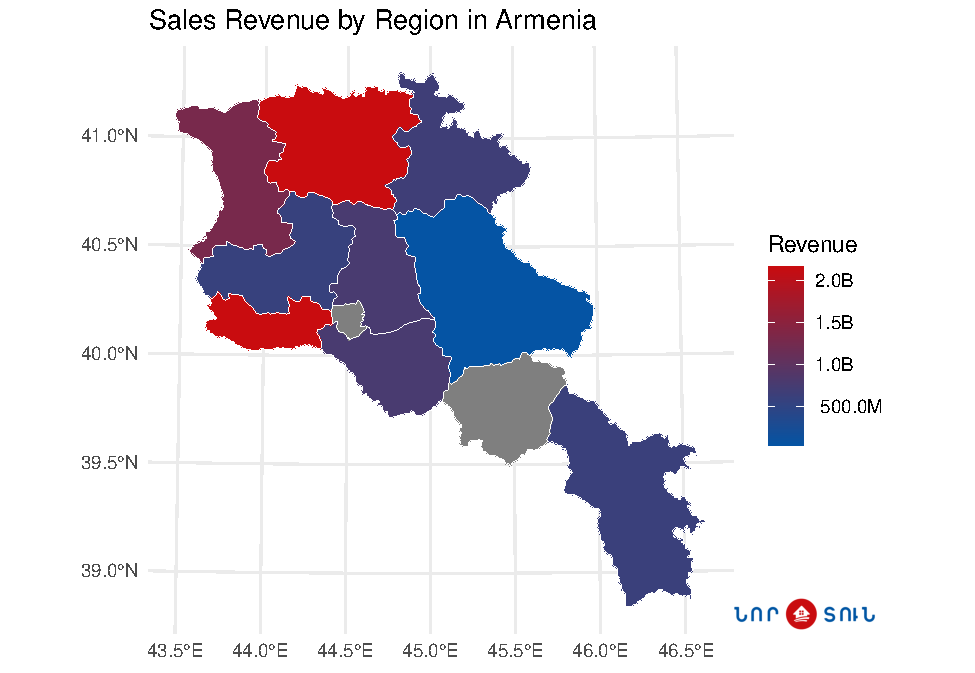
\includegraphics[width=\columnwidth,keepaspectratio]{./figures/sales_by_map_armenia.pdf}
\caption{Source \cite{mapArmenia}}
\label{fig:sales_by_map_armenia}
\end{figure}

\begin{figure}[htbp]
\centering
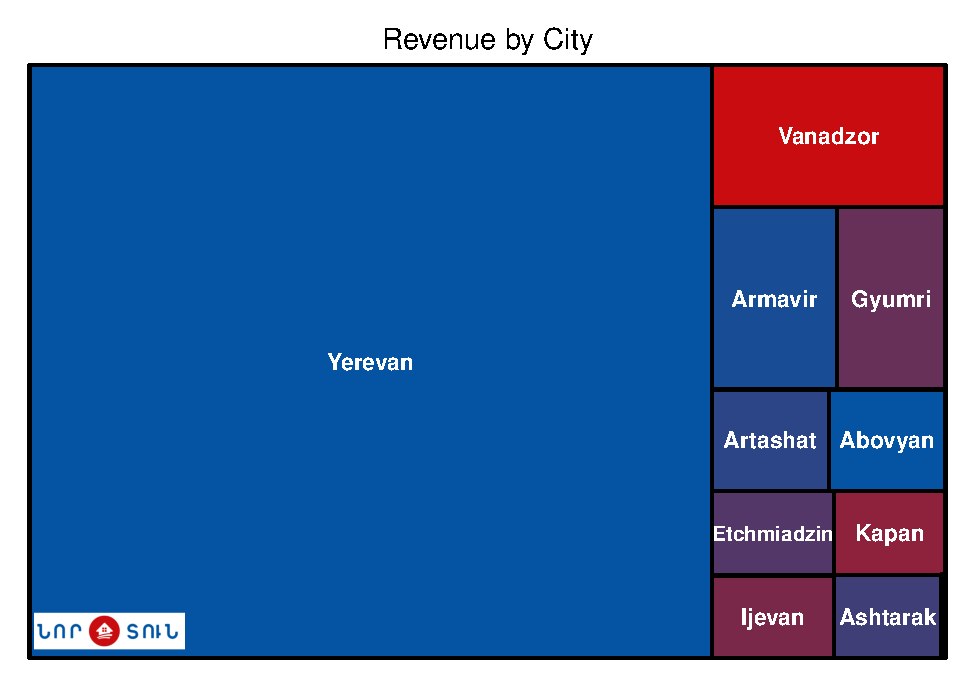
\includegraphics[width=\columnwidth,keepaspectratio]{./figures/treemap_whole.pdf}
\caption{Treemap of Shops by City Compared by Revenue \cite{treemap}}
\label{fig:treemap_whole}
\end{figure}

Outside of Yerevan, the best-performing shops are located in Vanadzor, Armavir, and Gyumri. (Figure~\ref{fig:sales_by_city}) The performance of the shops across different cities is explained by the size of the cities' populations. According to the Statistical Committee of the Republic of Armenia, the top 3 populated cities are Yerevan, Gyumri, and Vandazor. \cite{armstat2015}




Those are also the top-performing cities based on the revenue from the shops. The variation of sales performance across different regions of Armenia and Districts in Yerevan can be observed on the graph maps. (Figure~\ref{fig:sales_by_map_armenia} and Figure~\ref{fig:sales_by_map_yerevan}) 

\begin{figure}[htbp]
\centering
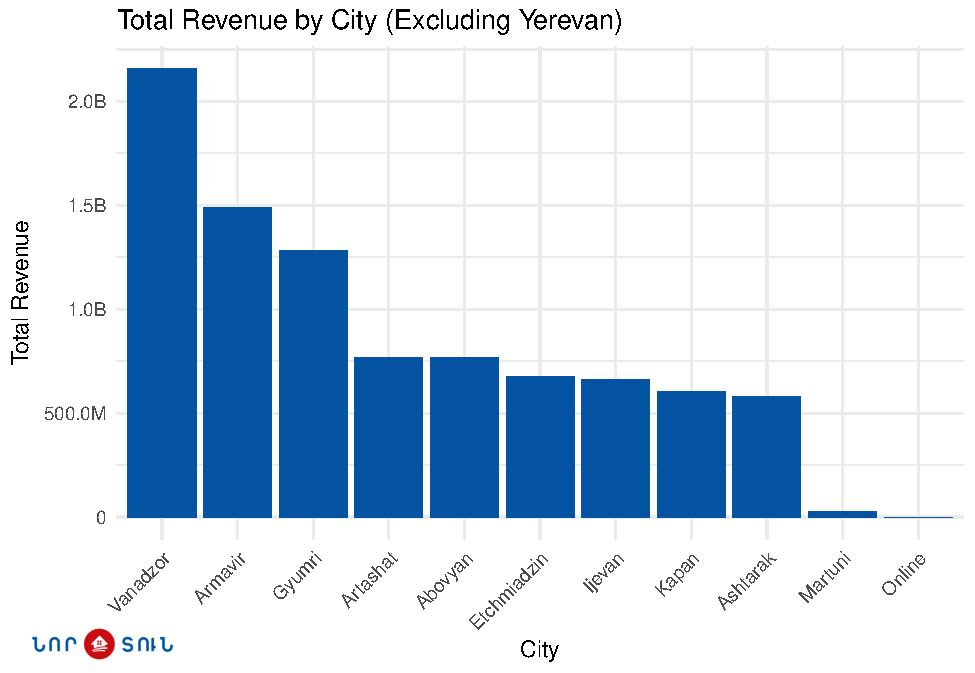
\includegraphics[width=\columnwidth,keepaspectratio]{./figures/sales_by_city.pdf}
\caption{Source \cite{SalesWithoutYerevan}}
\label{fig:sales_by_city}
\end{figure}


\begin{figure}[htbp]
\centering
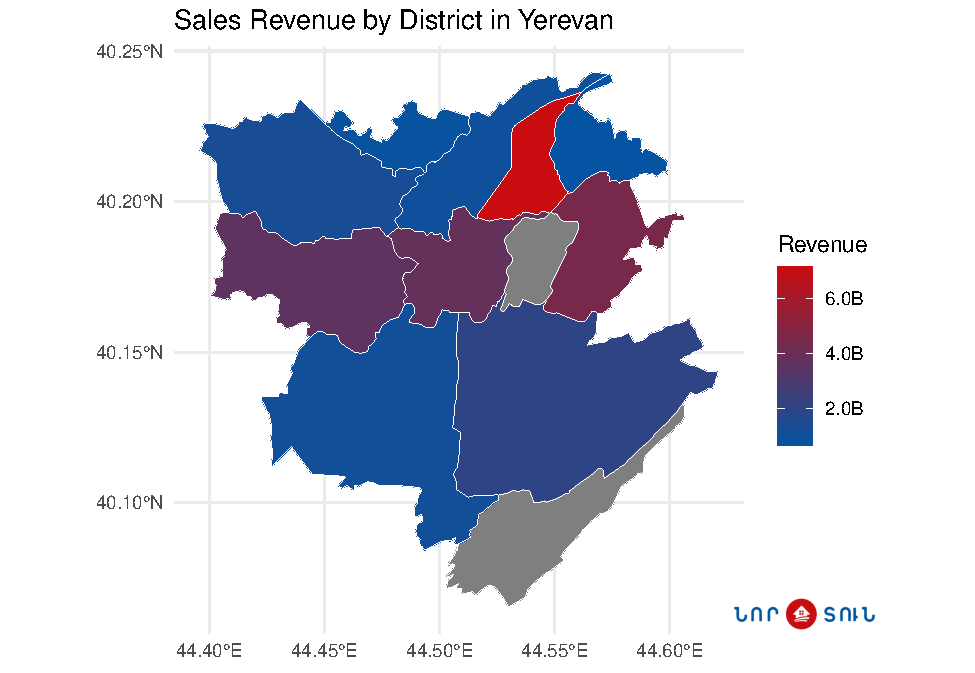
\includegraphics[width=\columnwidth,keepaspectratio]{./figures/sales_by_map_yerevan.pdf}
\caption{Source \cite{mapYerevan}}
\label{fig:sales_by_map_yerevan}
\end{figure}

\begin{figure}[htbp]
\centering
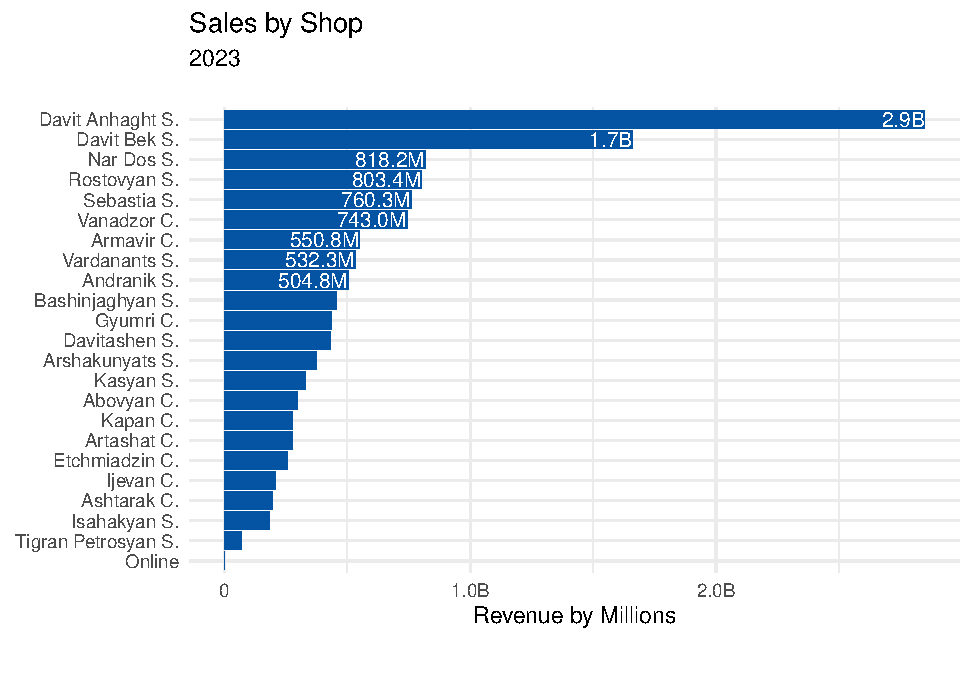
\includegraphics[width=\columnwidth,keepaspectratio]{./figures/sales_by_shop_2023_sales.pdf}
\caption{Source \cite{RevenuDistribution}}
\label{fig:sales_by_shop_2023}
\end{figure}

The distribution among all stores in 2023 can be seen in Figure~\ref{fig:sales_by_shop_2023} (The corresponding graph for 2022 and 2021 can be found in Appendix~\autoref{app:sales-distribution}). The Best-performing shop across all years is Davit Anhaght shop, which has significantly higher revenue than others. There has been significant growth in revenue at shops Nar-Dos and Rostovian in 2023 compared to previous years. The shops are now in the top 5 best-performing shops, which was not the case in previous years.

%  =====================================================================================================================================
%                                                       Product Category Analysis
%  =====================================================================================================================================

\subsection{Product Category Analysis}
Analysis of product categories and brands provides a clear understanding of consumer preferences. The performance of brands and categories of products are important factors of consideration for restocking and inventory management. From Figure~\ref{fig:number_revenue_comparison}, it can be observed that the largest quantity of products sold is in the category ``Other.'' 
\begin{figure}[htbp]
\centering
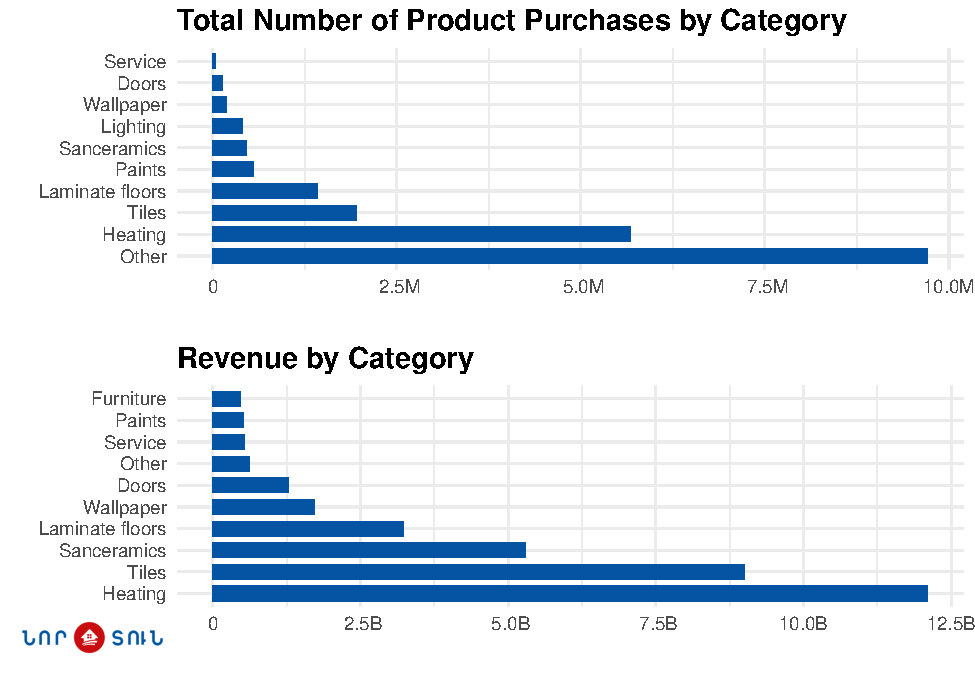
\includegraphics[width=\columnwidth,keepaspectratio]{./figures/revenue_quantity_comparison_by_category.pdf}
\caption{Source \cite{Categorygraph}}
\label{fig:number_revenue_comparison}
\end{figure}
This is very logical since this category includes small building materials and chemicals that are sold in large quantities. However, these are cheap products, and despite the volume of their sales, they do not produce significant revenue. The top performing categories in stores are heating and tiles, both in terms of sold quantity and generated revenue. Interestingly, the wallpapers are sold in fewer quantities than the paints, but they produce higher revenue than the paints. Since the best-performing products are heating products and tiles, it is important to know the top-performing brands in those categories (Figure~\ref{fig:top_5_tiles_heating}). For heating products, Kaldo is the best-performing brand. In the tiles category, the Stn Spain brand generates more than twice the revenue of the top second brand.
\begin{figure}[htbp]
\centering
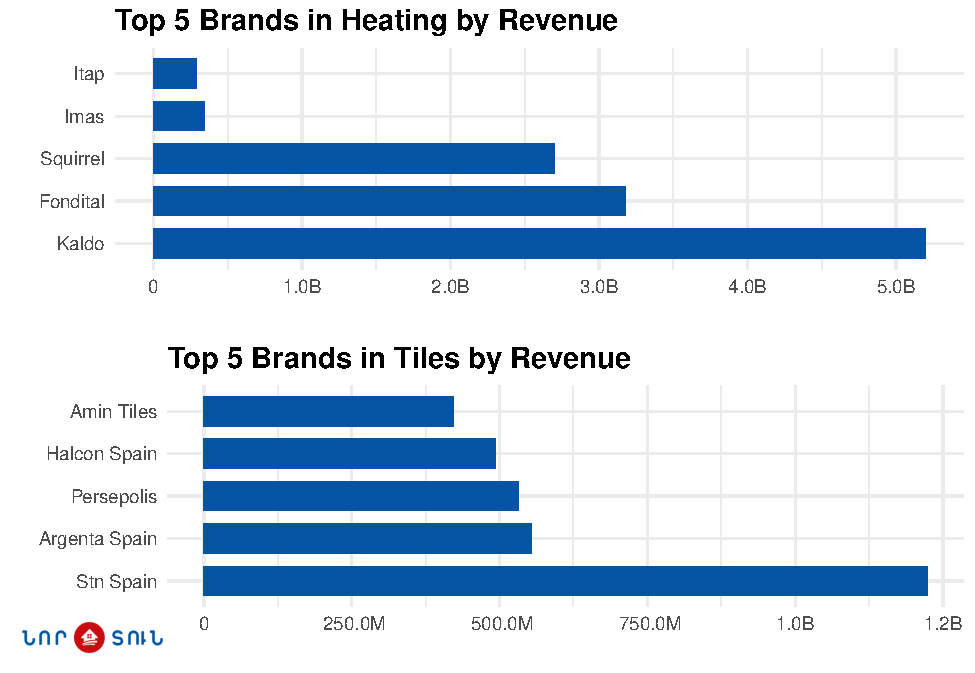
\includegraphics[width=\columnwidth,keepaspectratio]{./figures/top_5_tiles_heating.pdf}
\caption{Source \cite{TilesHeating}}
\label{fig:top_5_tiles_heating}
\end{figure}

%  =====================================================================================================================================
%                                                      Observations and Strategic Implications
%  =====================================================================================================================================

\subsection{Observations and Strategic Implications}
The key metrics of performance of the ``Nor Tun'' chain of stores have been identified in this section. The analysis suggests that there is a high divergence between the sales of various shops. Implementation of shop specific strategies and promotions can increase the performance of worse performing shops. 

The detected anomaly peak of the sales in 2023 shows that shops can perform unexpectedly well during the lowest seasons. Marketing campaigns should be implemented to increase sales during the lowest seasons and promote shops in various regions of Armenia.


%  =====================================================================================================================================
%                                                        Methodology and Results 
%  =====================================================================================================================================

\section{Methodology and Results}
The study aimed to find the best-performing time series sales forecasting (TSSF) models for accurately forecasting the future sales of ``Nor Tun'' chain stores. This section explains the models that were used for forecasting. Both univariate and multivariate forecasting methods were implemented and tested. Univariate forecasting aims to forecast overall sales across all stores combined, using only the historical sales data. Multivariate forecasting uses historical sales data, along with other attributes that were correlated with the sales, to perform forecasting for each store separately. Data preprocessing steps were applied to ensure the quality of the data passed to the models. The process includes handling missing values, feature scaling, and target encoding. The models were evaluated based on MAE, MAPE, RMSE, and R-squared metrics. A detailed description of these metrics can be found in Appendix~\autoref{app:metrics}.
% \usepackage{graphicx}
\begin{table}[]
\centering
\resizebox{\columnwidth}{!} & \textbf{46.25\%} & 89.08\%       & 50.16\%          \\
RMSE             & \textbf{8.143}   & \textbf{12.648}  & 12.829        & 15.250           \\
R Squared        & \textbf{0.801}   & \textbf{0.609}   & 0.506         & 0.432            \\ \hline
\end{tabular}%
}
\caption{ Performance Metrics for One Layer and Stacked LSTM Models. The MAE and RMSE values are presented in millions, e.g., an MAE of 6.03 represents 6,030,000.\cite{inferrence}}
\label{tab:lstm-table}
\end{table}

%  =====================================================================================================================================
%                                                      Univariate Forecasting: LSTM Models
%  =====================================================================================================================================

% \usepackage{booktabs}
% \usepackage{graphicx}
\begin{table*}[]
\centering
\resizebox{\textwidth}{!}{%
\begin{tabular}{@{}ccccccccccc@{}}
\toprule
                 & \multicolumn{2}{c}{Linear Regression} & \multicolumn{2}{c}{Decision Tree Regressor} & \multicolumn{2}{c}{Gradient Boosting Regressor} & \multicolumn{2}{c}{\textbf{Random Forest Regressor}} & \multicolumn{2}{c}{\textbf{XGBoost Regressor}} \\ \midrule
\textbf{Metrics} & Train             & Validation        & Train                  & Validation         & Train                & Validation               & Train                     & Validation               & Train                  & Validation            \\ \midrule
MAE              & 17364             & 16832             & \textbf{1001}          & 8267               & 10,005               & 9963                     & 2660                      & \textbf{6566}            & 6396                   & 6816                  \\
MAPE             & \textbf{4.6\%}    & \textbf{4.6\%}    & 31.3\%                 & 144\%              & 275\%                & 304\%                    & 45\%                      & 129\%                    & 120\%                  & 145\%                 \\
RMSE             & 69339             & 58682             & \textbf{7426}          & 41631              & 34686                & 33501                    & 19853                     & \textbf{31033}           & 22671                  & 33183                 \\
R Squared        & 0.338             & 0.392             & 0.992                  & 0.694              & 0.834                & 0.802                    & \textbf{0.946}            & \textbf{0.829}           & \textbf{0.929}         & \textbf{0.805}        \\ \bottomrule
\end{tabular}%
}
\caption{Performance Metrics Across Various Regression Models. \cite{inferrence}}
\label{tab:all-ml-table}
\end{table*}
\begin{figure}[htbp]
\centering
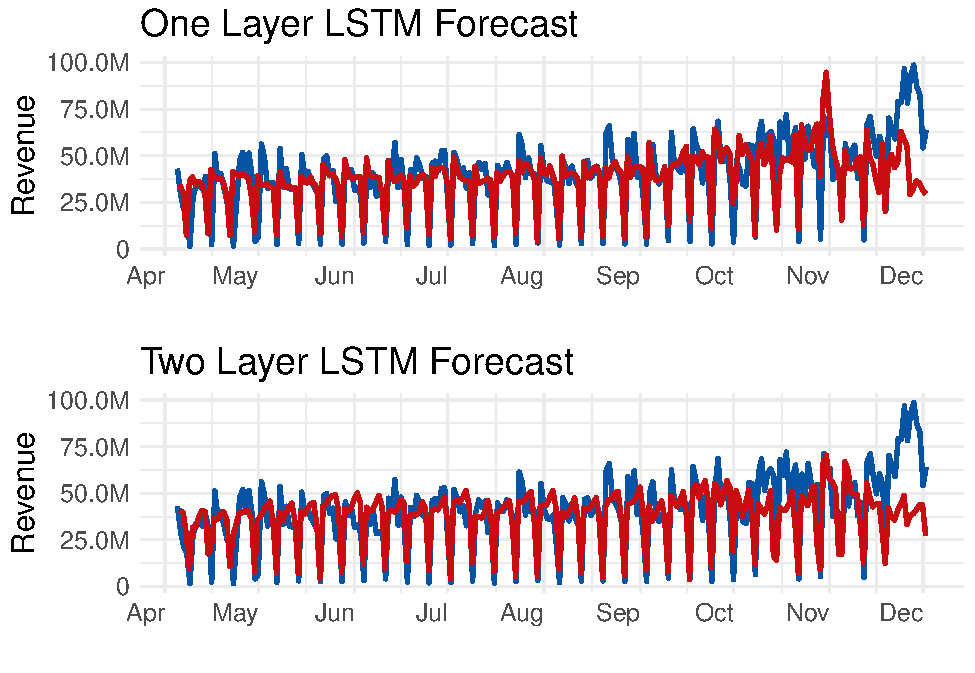
\includegraphics[width=\columnwidth,keepaspectratio]{./figures/lstm_predictions.pdf}
\caption{Forecasting result of both LSTM models \cite{lstmforecast}}
\label{fig:lstm_predictions}
\end{figure}
\subsection{Univariate Forecasting: LSTM Models}
Long Short-Term Memory (LSTM) models perform well on sequential data, and they are particularly useful for TSF tasks since they can capture different seasonal aspects of the data. The window size for the LSTM models was chosen by the trial method. Generally, it is a good practice to use the size of the seasonal pattern as a window size; in our case, it would be 7 since the seasonality of the data is weekly (see Figure~\ref{fig:time-series-2023}). However, after trying multiple window sizes, I found that a window size of 7 is too small for this model and is not capturing important long-term patterns. For the final model, a window size of 28 was chosen since it produced the best results for both LSTM models. The final hidden size of the models is 512. This size showed good results and, at the same time, did not make the model too heavy. One-layer and two-layer LSTM, known as stacked LSTM, were tested to find the appropriate model for the specific data. Adding a layer improves the ability of the model to capture deeper temporal patterns. In~\autoref{tab:lstm-table}, you can find a detailed evaluation of two LSTM networks using various metrics. As you can see, overall, the performance of one-layer LSTM is better than that of the stacked LSTM, both for training and validation sets. Overall, the model performance is not as good as it was expected (Figure~\ref{fig:lstm_predictions}). However, it is understandable since the model makes predictions based only on previous sales data without considering other variables. In the next section, we will see that the multivariate approach works better for this specific case.




%  =====================================================================================================================================
%                                                      Univariate Forecasting: Transformer Based Models
%  =====================================================================================================================================


\subsection{Univariate Forecasting: Transformer Based Models}
In recent years, transformer-based models have taken over the deep learning field. Originally, transformer models were used for NLP tasks, but it was later found that they perform well on any sequential data. Now, transformer models are used in any field where data can be tokenized and represented in sequential form. The attention mechanisms used in transformer models allow the model to determine the relevance of different parts of the data for a specific point. However, transformer models have shortcomings, the most important of which is that they are computationally expensive and require powerful machines. To overcome this problem, it is common practice to use pre-trained transformer models and fine-tune them for a specific task. In this project, I used a pre-trained Lag-Llama model, which is a decoder-only transformer with zero-shot prediction capabilities. Lag-Llama is a probabilistic model, which means that the model predicts not just single-point estimates but a distribution of possible outcomes. In the next step, the model chooses the median point of the distribution and uses it as a prediction for that time point. For both zero-shot and fine-tuned models, I set the prediction size to 1000 for a one-time point. For each time point, the model makes a distribution of predictions consisting of 1000 points and takes the median as the final prediction point. From~\autoref{tab:Lag_llama_table}, you can clearly observe that the model's forecasting ability increases drastically after fine-tuning. Additionally, the fine-tuned Lag-Llama model is showing the best performance across all univariate models (Figure~\ref{fig:lag_llama_predictions}). The results can be observed on the graphs Figure X and Figure Y as well.
% Please add the following required packages to your document preamble:
% \usepackage{graphicx}
\begin{table}[]
\centering
\resizebox{\columnwidth}{!} & 170.7  \\
RMSE & \textbf{15.702}   & 21.893 \\ \hline
\end{tabular}%
}
\caption{ Performance Comparison Between Fine-Tuned and Zero-Shot Inference. The MAE and RMSE values are presented in millions, e.g., an MAE of 1.831 represents 1,831,000. \cite{inferrence_lag_llama}}
\label{tab:Lag_llama_table}
\end{table}

\begin{figure}[htbp]
\centering
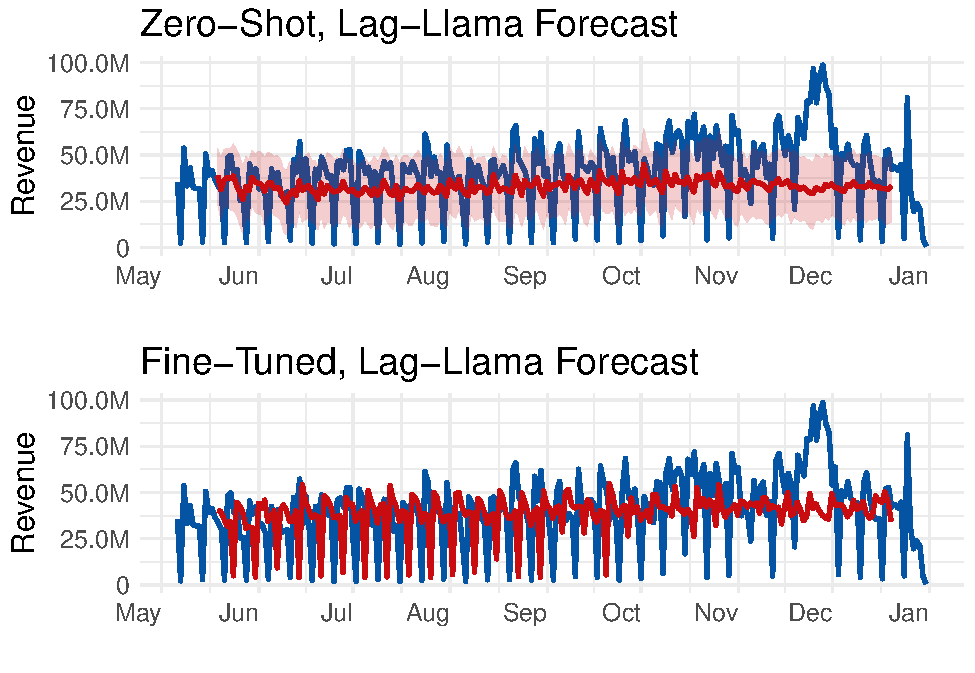
\includegraphics[width=\columnwidth,keepaspectratio]{./figures/lag_llam_prediction.pdf}
\caption{Forecasting result of both Zero-Shot and Fine-Tuned models \cite{lagllamaforecast}}
\label{fig:lag_llama_predictions}
\end{figure}

%  =====================================================================================================================================
%                                                      Multivariate Forecasting: Machine Learning Models
%  =====================================================================================================================================

\subsection{Multivariate Forecasting: Machine Learning Models}
In addition to univariate models, a multivariate approach was implemented for forecasting. This approach helped to obtain predictions for each store separately. For this part, I utilized machine learning models to compare the performances of multiple models. Before the implementation of the models, a feature selection process was conducted, which is described in detail in the future engineering part of the paper. Since the majority of features were categorical, it was necessary to transform them into meaningful numerical values. Target encoding was used for this purpose. The encoder was fitted on train data and then applied to validation and test sets. This approach helps to avoid data leakage. Five different models were evaluated before choosing the final model. When a model performs well on a training dataset, it can indicate overfitting, and the model will later fail to generalize. Computing the performance on the validation set ensures that the model can be generalized. The results of the models can be found in Table X. Some models showed excellent results on the training dataset but failed to generalize and make good predictions on the validation dataset. 
Based on the performance on both test and validation datasets, Random Forest Regressor and XGBoost were selected (~\autoref{tab:all-ml-table}). These two models were then combined using an ensemble technique. Best performing models were stacked using a stacking regressor. This method was expected to decrease the error given that two models are independent and diverse. As you can see from ~\autoref{tab:final-ml}, this approach was not successful. The Stacking regressor performed well but did not surpass base models. Since the Random Forest Regressor outperformed all the other models, it was chosen as the final model. You can see the predictions of this model in Figure~\ref{fig:RFR_predictions}.
% \usepackage{booktabs}
% \usepackage{graphicx}
\begin{table}[]
\centering
\resizebox{\columnwidth}{!}{%
\begin{tabular}{@{}cllcccc@{}}
\toprule
 &
  \multicolumn{2}{c}{\textbf{Stacking Regressor}} &
  \multicolumn{2}{c}{XGBoost Regressor} &
  \multicolumn{2}{c}{\textbf{Random Forest Regressor}} \\ \midrule
\textbf{Metrics} &
  \multicolumn{1}{c}{Train} &
  \multicolumn{1}{c}{Validation} &
  Train &
  Validation &
  Train &
  Validation \\ \midrule
MAE       & 3946  & 7253  & 6396  & 6816  & \textbf{2660}  & \textbf{6566}  \\
MAPE      & 174\% & 278\% & 120\% & 145\% & \textbf{45\%}  & \textbf{129\%} \\
RMSE      & 28064 & 31956 & 22671 & 33183 & \textbf{19853} & \textbf{31033} \\
R Squared & 0.892 & 0.820 & 0.929 & 0.805 & \textbf{0.946} & \textbf{0.829} \\ \bottomrule
\end{tabular}%
}
\caption{Stacked Regression Model Versus Individual Models: Choosing Final Model. \cite{inferrence}}
\label{tab:final-ml}
\end{table}

\begin{figure}[htbp]
\centering
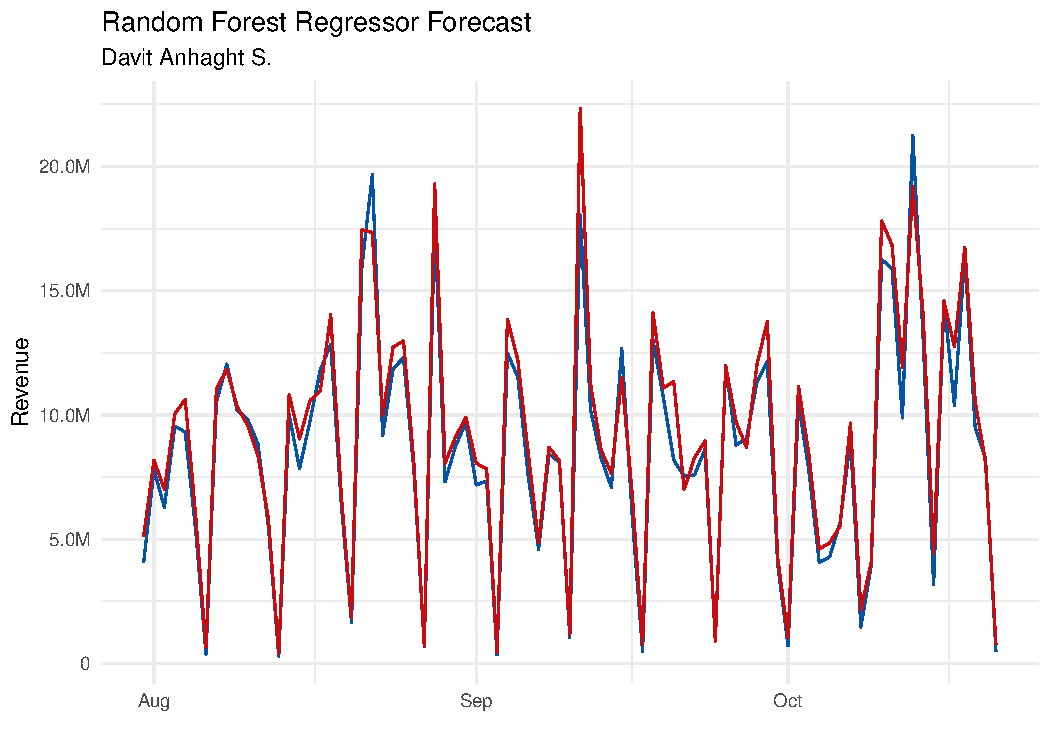
\includegraphics[width=\columnwidth,keepaspectratio]{./figures/ML_davit_anhaght_prediction.pdf}
\caption{Source \cite{MLforecast}}
\label{fig:RFR_predictions}
\end{figure}

%  =====================================================================================================================================
%                                                      Conclusion and Discussion
%  =====================================================================================================================================

\section{Conclusion and Discussion}
This research successfully demonstrated the efficiency of various time series forecasting techniques that are performing well in the specific case of “Nor Tun” chain stores. Among the tested models fine tuned lag-llama model showed excellent performance, highlighting the strength of modern transformer based models. 

Machine learning models, tested for multivariate forecasting, showed the efficiency of ensemble models, particularly of XGBoost and Random Forest Regressor. 

The sales analysis highlighted key best-performing metrics of the “Nor Tun” chain stores. Based on analysis, I made recommendations, to improve the performance of shops with lowest performance, and increase sales during low seasons. 

This study aims to become the starting point for the “Nor Tun” chain stores, business research. There is a big potential to conduct additional research, and integrate modern ML mechanisms into the business, to improve the performance. This research not only advances the academic field of applied time series forecasting but also provides meaningful insights to the BARSIS LLC that could be directly applied to business processes.

\section*{Acknowledgment}
I would like to thank BARSIS LLC for providing their private information for academic research and my supervisor for guidance.

%  =====================================================================================================================================
%                                                       References
%  =====================================================================================================================================

\bibliographystyle{IEEEtran}
\bibliography{references}

%  =====================================================================================================================================
%                                                       Appendix
%  =====================================================================================================================================

\newpage % Ensure the appendix starts on a new page
\appendices

\section{ANOVA analysis}
\label{app:anova}
Anova analysis was chosen to identify the relationship between continuous target variables and categorical independent variables. One-way ANOVA compares sample means of continuous variables across all categories within the categorical variable. If there are three categories of categorical variables, then we will get three means, $\mu_0,\mu_1,\mu_2 $ each representing the mean of continuous variables for that specific category. This test aims to find whether a categorical variable influences the distribution of continuous variables or not. The assumption is the following: if the categorical variable has no influence over the continuous variable, then the mean of the three samples should be identical($\mu_0=\mu_1=\mu_2 $). If the means are not identical, it means that the categorical variable has a strong influence on the variance of the continuous variable.

\section{Day-to-Day Sales in 2021 and 2022}
\label{app:time-series}
\begin{figure}[htbp]
\centering
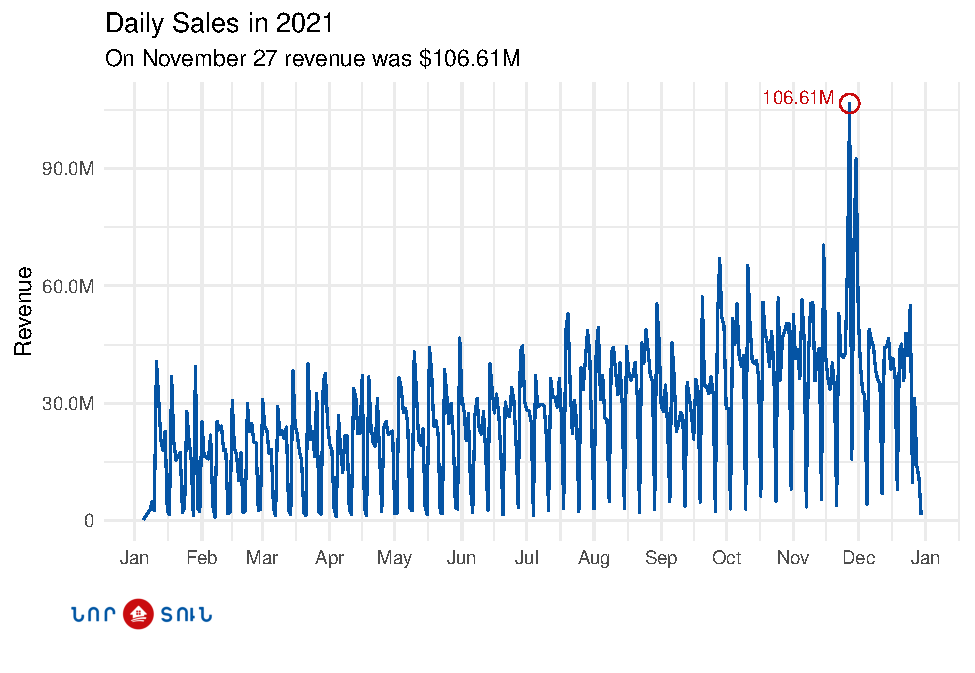
\includegraphics[width=\columnwidth,keepaspectratio]{./figures/time_series_2021_sales.pdf}
\caption{Source \cite{TSF}}
\label{fig:time-series-2021}
\end{figure}


\begin{figure}[htbp]
\centering
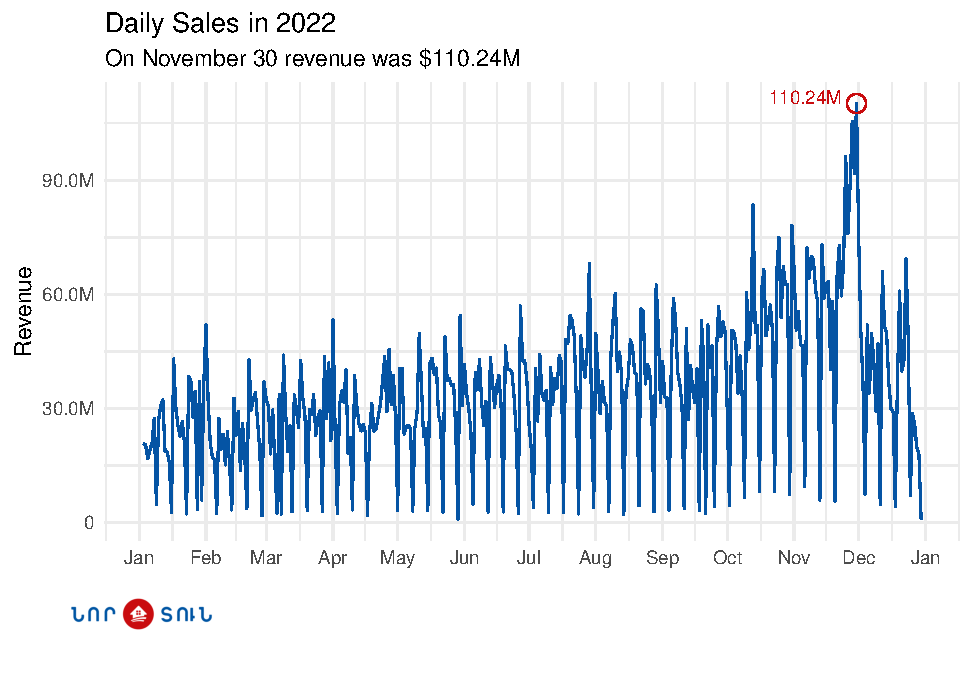
\includegraphics[width=\columnwidth,keepaspectratio]{./figures/time_series_2022_sales.pdf}
\caption{\cite{TSF}}
\label{fig:time-series-2022}
\end{figure}

\section{Distribution of generated revenue among all stores in 2021 and 2022}
\label{app:sales-distribution}
\begin{figure}[htbp]
\centering
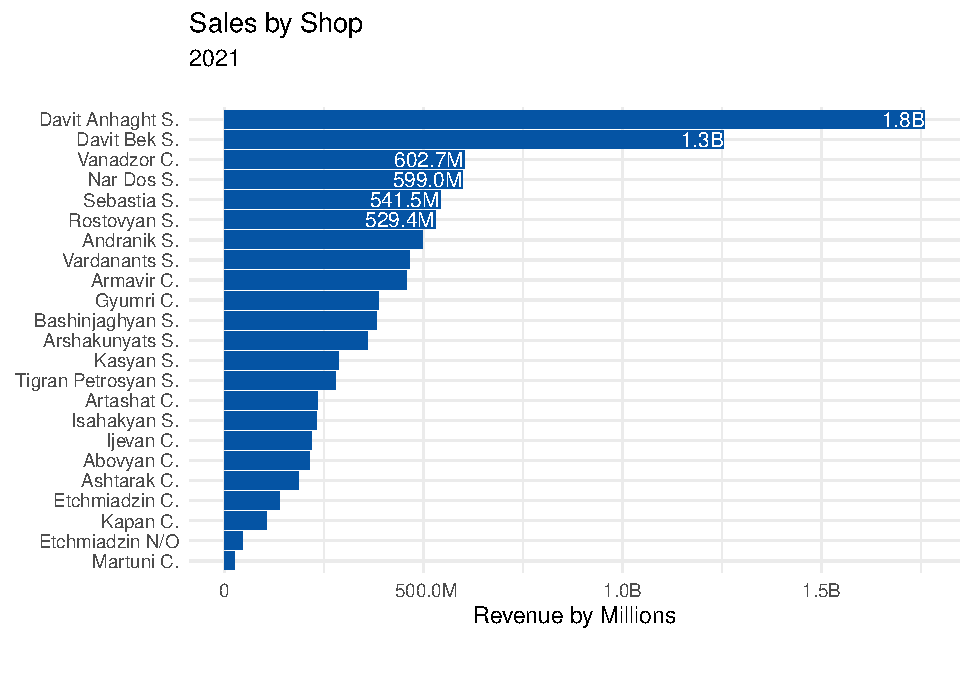
\includegraphics[width=\columnwidth,keepaspectratio]{./figures/sales_by_shop_2021_sales.pdf}
\caption{\cite{RevenuDistribution}}
\label{fig:sales-by-shop-2021}
\end{figure}


\begin{figure}[htbp]
\centering
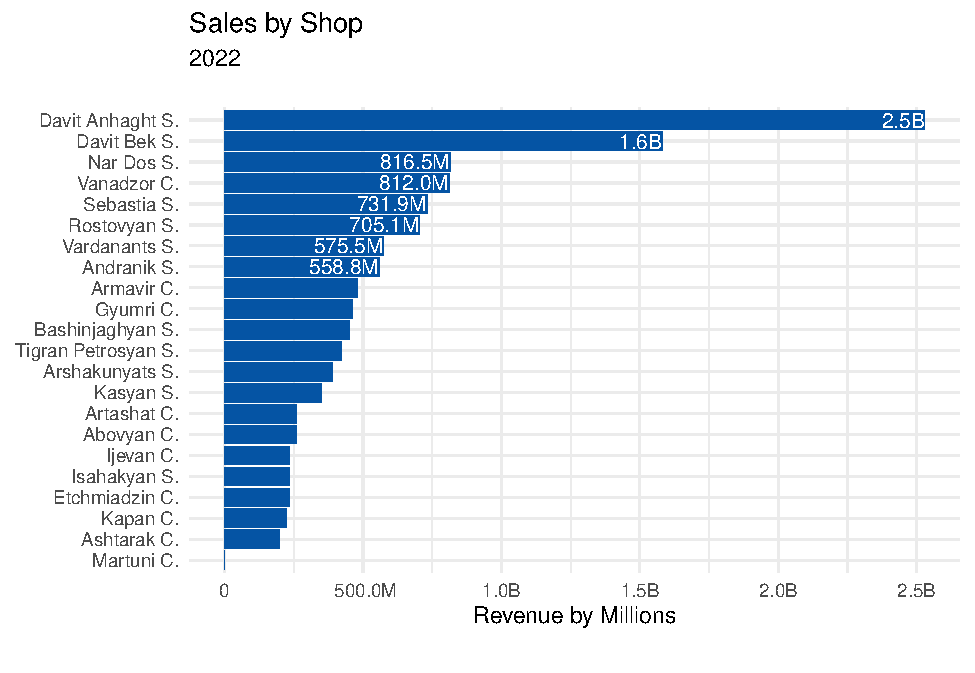
\includegraphics[width=\columnwidth,keepaspectratio]{./figures/sales_by_shop_2022_sales.pdf}
\caption{Source \cite{RevenuDistribution}}
\label{fig:sales-by-shop-2022}
\end{figure}


\section{Explanation of metrics}
\label{app:metrics}
\subsection{MAE}
The mean absolute error is a measure of the difference between a certain observation's forecast and its real value. MAE computes the average of absolute errors for a set of observations and predictions to determine the proportion of the errors for the entire group. 
$$MAE = \frac{1}{n}\sum_{i=1}^n|(y_i - \hat{y_i})|$$

\subsection{MAPE}
Mean absolute percentage error (MAPE) is a statistical metric used to assess the precision of a forecasting technique. It is the average of the absolute percentage errors of each item in a dataset that determines how precise the predicted proportions were in contrast to the true values. 
$$MAPE = 100\frac{1}{n}\sum_{i=1}^n\Bigg|\frac{(y_i - \hat{y_i})}{\hat{y_i})}\Bigg|$$

\subsection{RMSE}
The Root Mean Square Error is the standard deviation of the residuals prediction errors. Prediction errors represent the distance between data points and the regression line.
$$RMSE  = \sqrt{\frac{1}{n}\sum_{i=1}^n(y_i - \hat{y_i})^2}$$
\subsection{R-squared}
R-squared is a statistical metric that shows how much variance in a dependent variable is explained by an independent variable in a regression model. It is a goodness-of-fit metric for linear regression models. Greater R-squared values indicate a more accurate fit, but this does not always imply that the model is a strong predictor in absolute terms.
$$R^2  = 1 - \frac{\sum_{i=1}^n(y_i - \hat{y_i})^2}{\sum_{i=1}^n(y_i - \bar{y_i})^2}$$
\end{document}
